% ADAS map-generation workflow (kitti-seq04) — presentation figure.
% Compile:  pdflatex docs/mapgen_workflow.tex   (or tectonic / latexmk)
% Reuse in beamer: paste the tikzpicture, or \input the body.
\documentclass[border=10pt]{standalone}
\usepackage{tikz}
\usetikzlibrary{arrows.meta,positioning,fit,backgrounds,calc}

\definecolor{cInput}{HTML}{E8F0FE}
\definecolor{cPerc}{HTML}{FDE9D9}
\definecolor{cLift}{HTML}{E2F0D9}
\definecolor{cGeo}{HTML}{FFF2CC}
\definecolor{cAsm}{HTML}{F4CCCC}
\definecolor{cResult}{HTML}{D9D2E9}
\definecolor{cGen}{HTML}{ECECEC}

\begin{document}
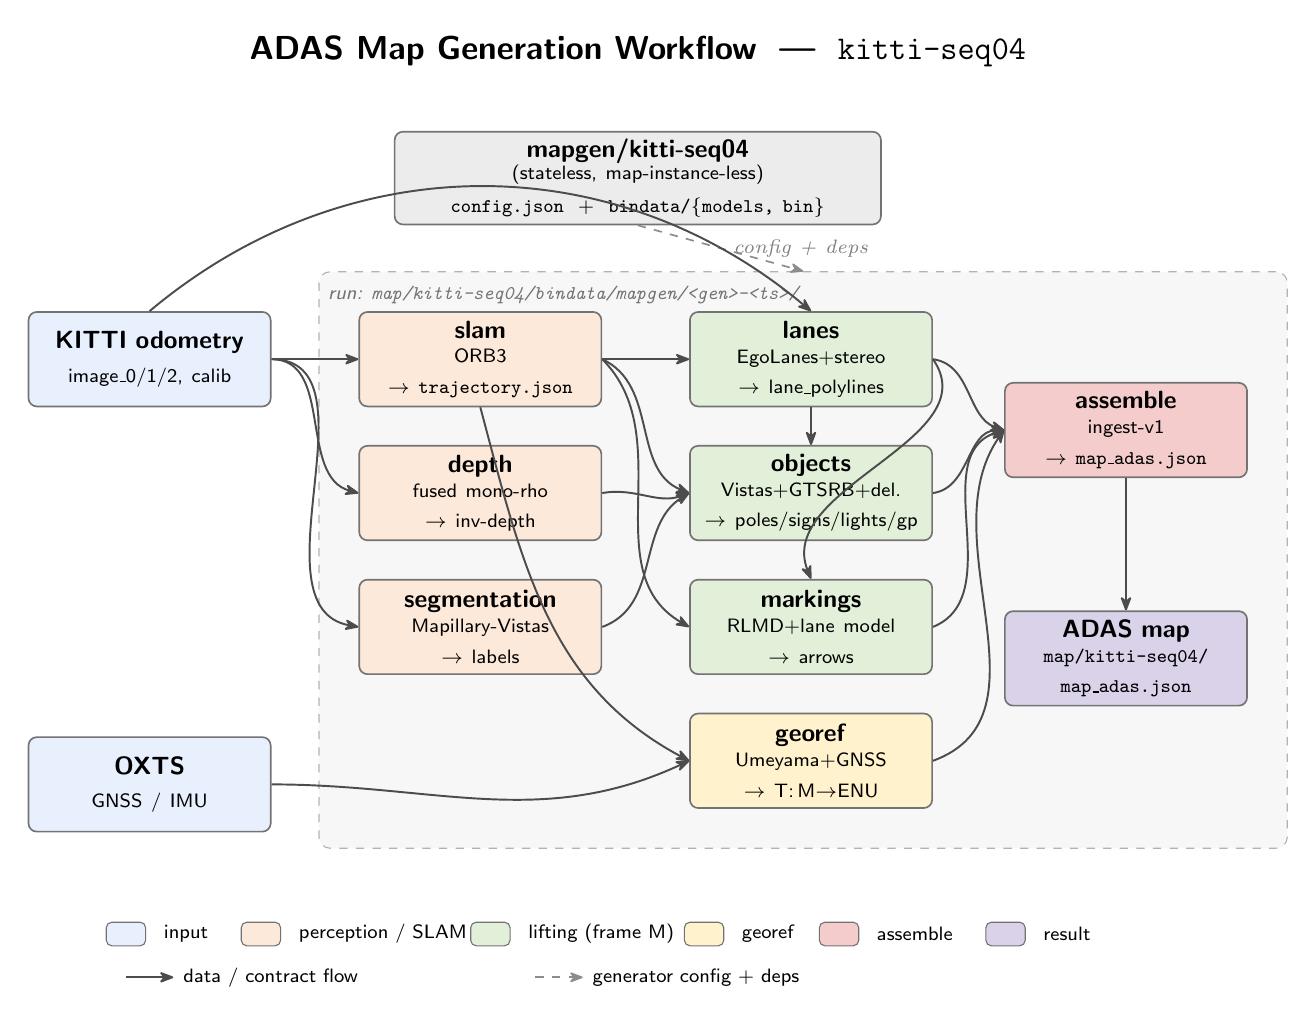
\begin{tikzpicture}[
  font=\sffamily\small,
  >={Stealth[round]},
  box/.style={rounded corners=3pt, draw=black!55, line width=.6pt, align=center,
              text width=29mm, minimum height=12mm, inner sep=2.5pt},
  arr/.style={->, line width=.7pt, draw=black!70},
  dep/.style={->, dashed, line width=.6pt, draw=black!45},
  legkey/.style={draw=black!55, rounded corners=2pt, minimum width=5mm, minimum height=3mm},
]

% ---- title ----
\node[font=\sffamily\bfseries\large] at (6.2,5.3)
  {ADAS Map Generation Workflow \;\textemdash\; \texttt{kitti-seq04}};

% ---- generator (stateless) ----
\node[box, fill=cGen, text width=60mm, minimum height=10mm] (gen) at (6.2,3.7)
  {\textbf{mapgen/kitti-seq04}\, \scriptsize(stateless, map-instance-less)\\[1pt]
   \scriptsize \texttt{config.json} \;+\; \texttt{bindata/\{models, bin\}}};

% ---- inputs (map state) ----
\node[box, fill=cInput] (imgs) at (0,1.4)  {\textbf{KITTI odometry}\\[1pt]\scriptsize image\_0/1/2, calib};
\node[box, fill=cInput] (gnss) at (0,-4.0) {\textbf{OXTS}\\[1pt]\scriptsize GNSS / IMU};

% ---- perception + slam ----
\node[box, fill=cPerc] (slam)  at (4.2,1.4)  {\textbf{slam}\\[1pt]\scriptsize ORB3\\ $\to$ \texttt{trajectory.json}};
\node[box, fill=cPerc] (depth) at (4.2,-0.3) {\textbf{depth}\\[1pt]\scriptsize fused mono-rho\\ $\to$ inv-depth};
\node[box, fill=cPerc] (seg)   at (4.2,-2.0) {\textbf{segmentation}\\[1pt]\scriptsize Mapillary-Vistas\\ $\to$ labels};

% ---- lifting into world frame M (+ georef as 4th branch) ----
\node[box, fill=cLift] (lanes)    at (8.4,1.4)  {\textbf{lanes}\\[1pt]\scriptsize EgoLanes+stereo\\ $\to$ lane\_polylines};
\node[box, fill=cLift] (objects)  at (8.4,-0.3) {\textbf{objects}\\[1pt]\scriptsize Vistas+GTSRB+del.\\ $\to$ poles/signs/lights/gp};
\node[box, fill=cLift] (markings) at (8.4,-2.0) {\textbf{markings}\\[1pt]\scriptsize RLMD+lane model\\ $\to$ arrows};
\node[box, fill=cGeo]  (georef)   at (8.4,-3.7) {\textbf{georef}\\[1pt]\scriptsize Umeyama+GNSS\\ $\to$ T:\,M$\to$ENU};

% ---- assemble + result ----
\node[box, fill=cAsm]    (asm) at (12.4,0.5)  {\textbf{assemble}\\[1pt]\scriptsize ingest-v1\\ $\to$ \texttt{map\_adas.json}};
\node[box, fill=cResult] (map) at (12.4,-2.4) {\textbf{ADAS map}\\[1pt]\scriptsize \texttt{map/kitti-seq04/}\\ \texttt{map\_adas.json}};

% ---- run container (background) ----
\begin{scope}[on background layer]
  \node[draw=black!30, dashed, rounded corners=4pt, fill=black!3,
        fit=(slam)(seg)(lanes)(georef)(asm)(map), inner sep=5mm] (run) {};
  \node[anchor=north west, font=\sffamily\scriptsize\itshape, text=black!55]
        at ([yshift=-0.6mm]run.north west) {run: \texttt{map/kitti-seq04/bindata/mapgen/<gen>-<ts>/}};
\end{scope}
\draw[dep] (gen.south) -- node[right=1pt, font=\scriptsize\itshape, text=black!50] {config + deps} (run.north);

% ---- data / contract flow ----
\draw[arr] (imgs.east) -- (slam.west);
\draw[arr] (imgs.east) to[out=0,in=165]  (depth.west);
\draw[arr] (imgs.east) to[out=0,in=170]  (seg.west);
\draw[arr] (imgs.north) to[out=40,in=140] (lanes.north);

\draw[arr] (slam.east) -- (lanes.west);
\draw[arr] (slam.east) to[out=-25,in=158] (objects.west);
\draw[arr] (slam.east) to[out=-45,in=150] (markings.west);
\draw[arr] (slam.south) to[out=-75,in=152] (georef.west);
\draw[arr] (depth.east) to[out=10,in=200]  (objects.west);
\draw[arr] (seg.east)   to[out=20,in=212]  (objects.west);
\draw[arr] (lanes.south) -- (objects.north);
\draw[arr] (lanes.east)  to[out=-55,in=112] (markings.north);
\draw[arr] (gnss.east)   to[out=0,in=205]   (georef.west);

\draw[arr] (lanes.east)    to[out=-8,in=162] (asm.west);
\draw[arr] (objects.east)  to[out=8,in=182]  (asm.west);
\draw[arr] (markings.east) to[out=22,in=198] (asm.west);
\draw[arr] (georef.east)   to[out=20,in=235] (asm.west);
\draw[arr] (asm.south) -- (map.north);

% ---- legend ----
\begin{scope}[shift={(-0.3,-5.9)}, font=\sffamily\scriptsize]
  \node[legkey, fill=cInput]  (l1) {}; \node[right=1mm of l1] (t1) {input};
  \node[legkey, fill=cPerc, right=12mm of l1]  (l2) {}; \node[right=1mm of l2] (t2) {perception / SLAM};
  \node[legkey, fill=cLift, right=24mm of l2]  (l3) {}; \node[right=1mm of l3] (t3) {lifting (frame M)};
  \node[legkey, fill=cGeo, right=22mm of l3]   (l4) {}; \node[right=1mm of l4] (t4) {georef};
  \node[legkey, fill=cAsm, right=12mm of l4]   (l5) {}; \node[right=1mm of l5] (t5) {assemble};
  \node[legkey, fill=cResult, right=16mm of l5](l6) {}; \node[right=1mm of l6] (t6) {result};
  \draw[arr] (0,-0.55) -- ++(6mm,0) node[right, black] {data / contract flow};
  \draw[dep] (52mm,-0.55) -- ++(6mm,0) node[right, black] {generator config + deps};
\end{scope}

\end{tikzpicture}
\end{document}
